
\begin{figure}[H]
    \centering
    \begin{subfigure}[b]{0.49\textwidth}
        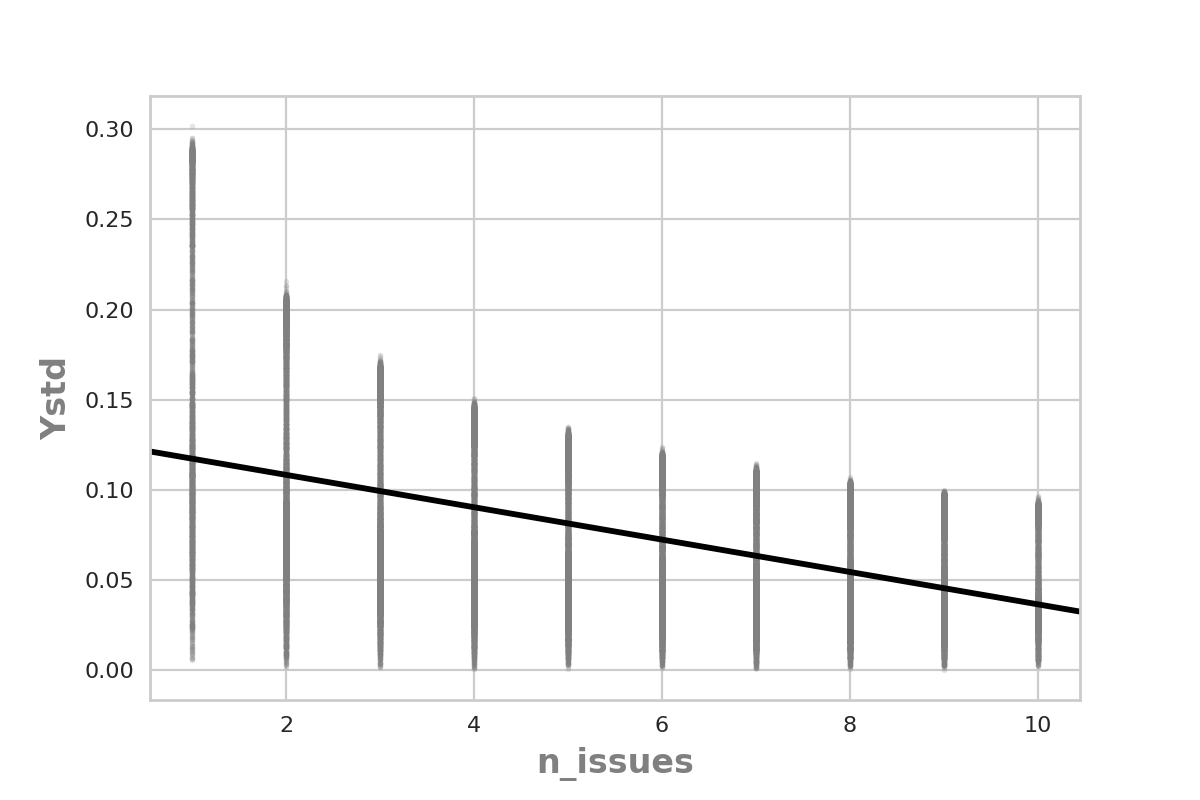
\includegraphics[width=\textwidth]{ims/sigmaregression/sigmaissues.png}
    \end{subfigure}
    \begin{subfigure}[b]{0.49\textwidth}
        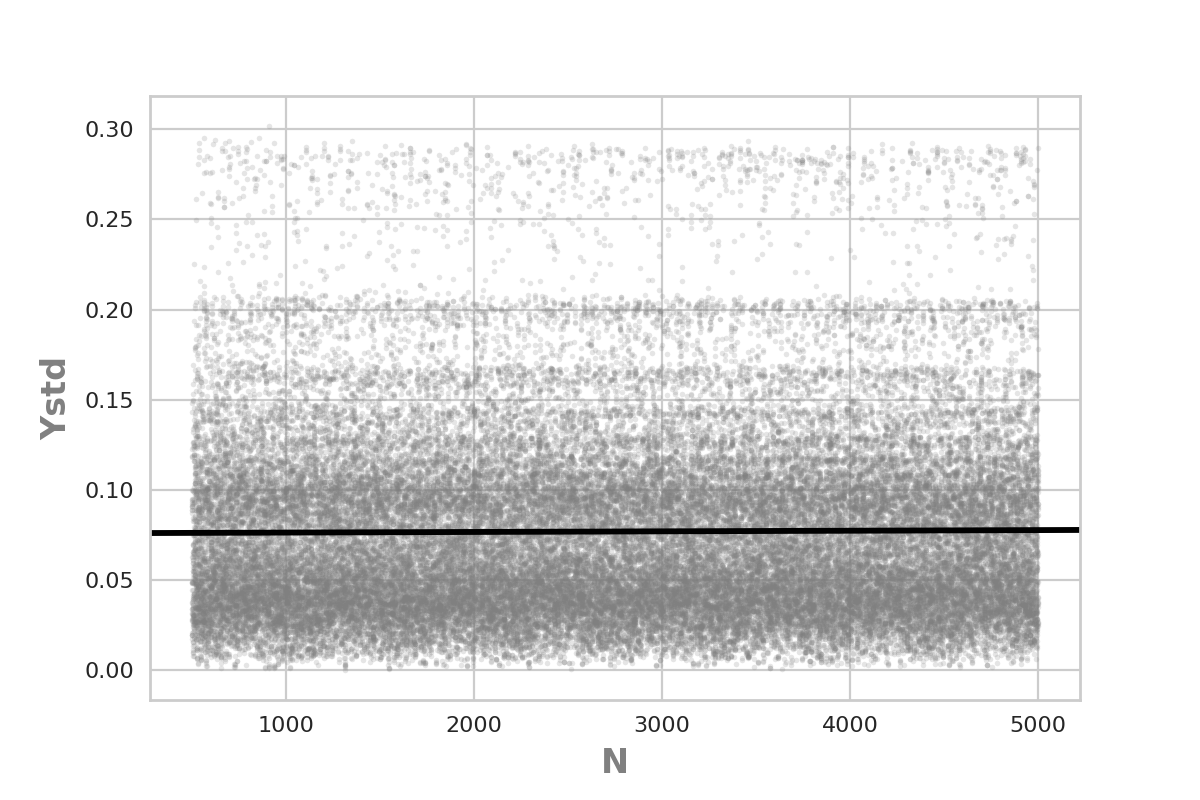
\includegraphics[width=\textwidth]{ims/sigmaregression/sigmaN.png}
    \end{subfigure}

    \begin{subfigure}[b]{0.49\textwidth}
        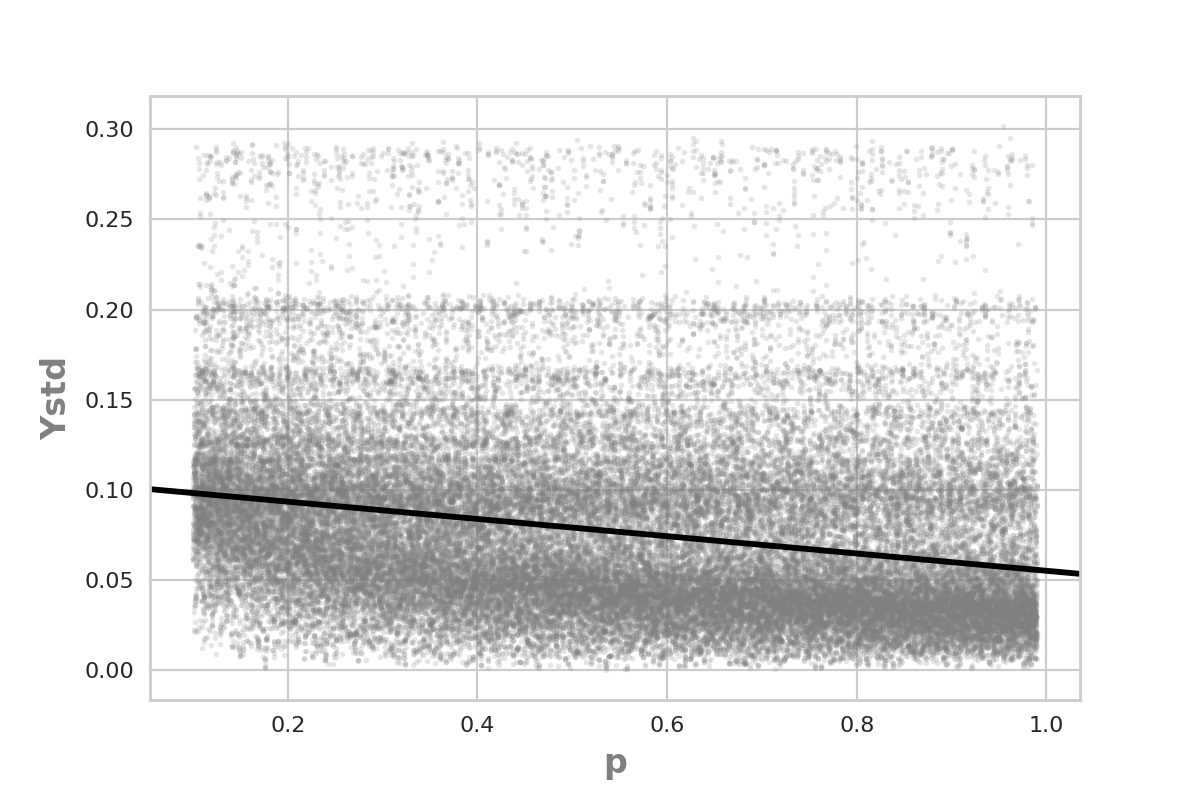
\includegraphics[width=\textwidth]{ims/sigmaregression/sigmap.png}
      \end{subfigure}
          \begin{subfigure}[b]{0.49\textwidth}
            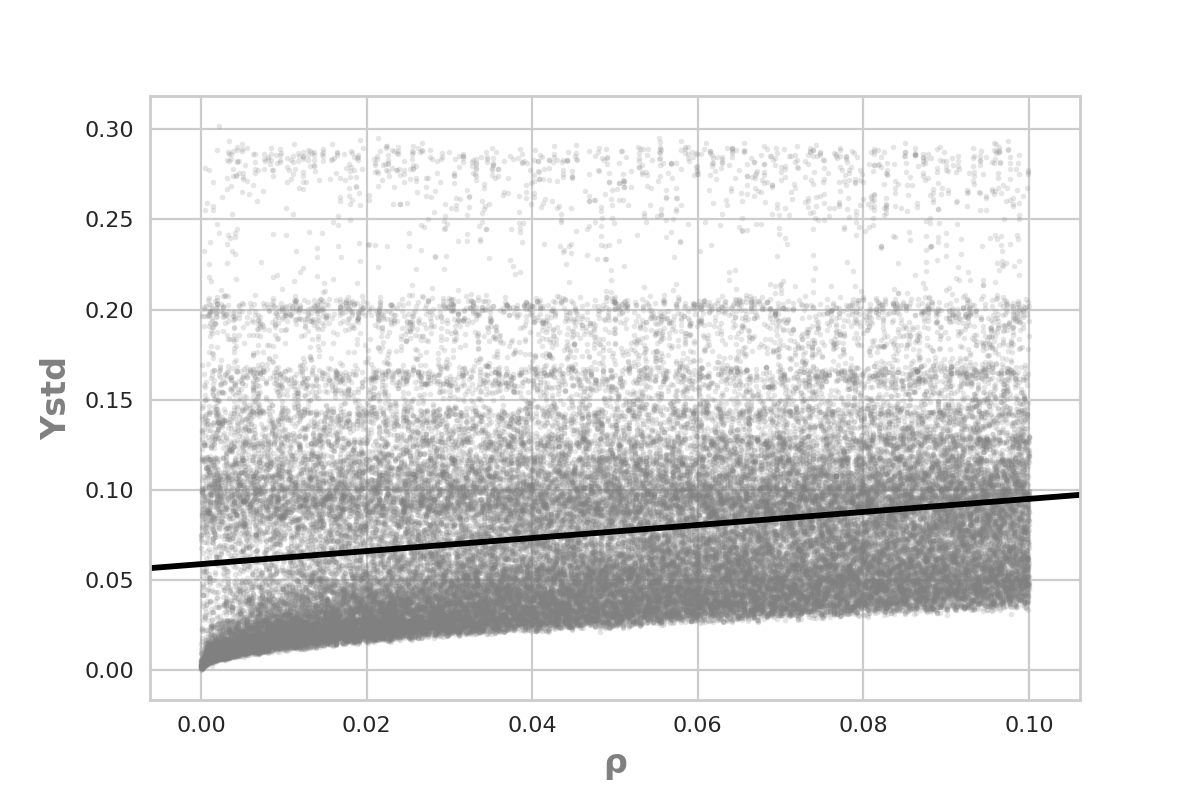
\includegraphics[width=\textwidth]{ims/sigmaregression/sigmarho.png}
      \end{subfigure}

                \begin{subfigure}[b]{0.49\textwidth}
            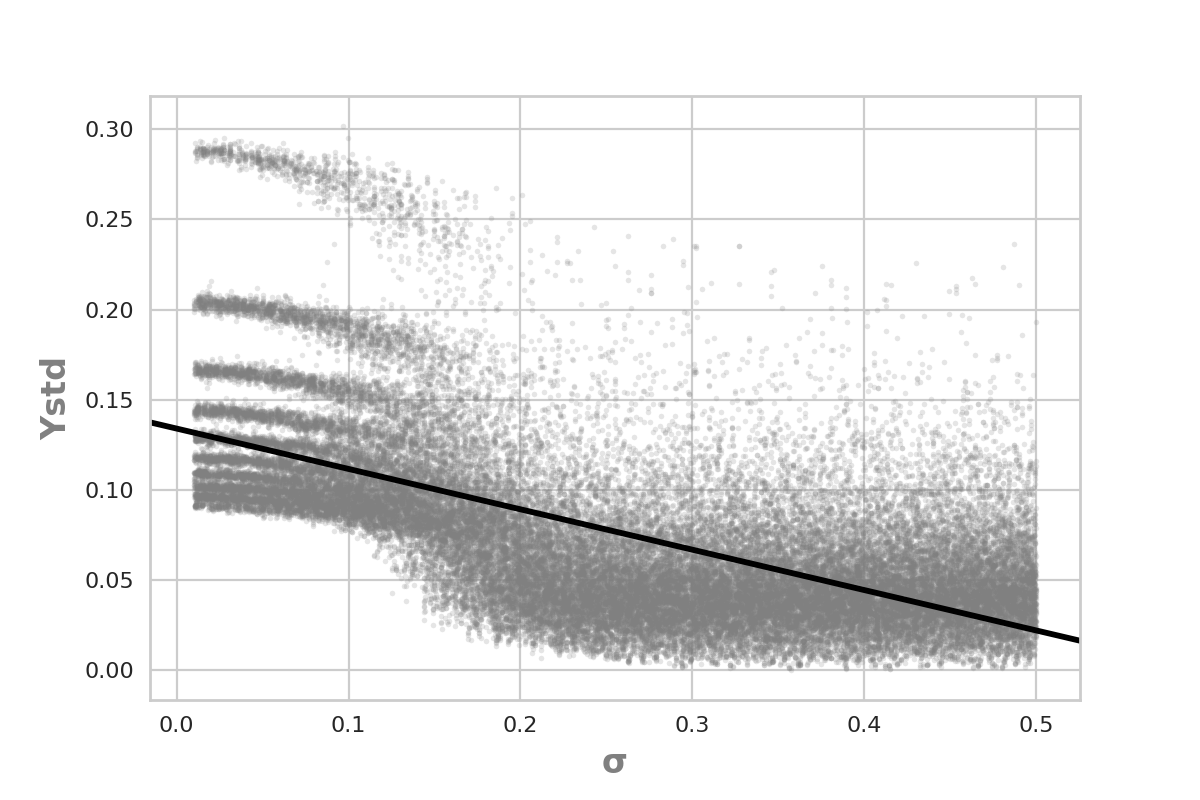
\includegraphics[width=\textwidth]{ims/sigmaregression/sigmasigma.png}
    \end{subfigure}
    \caption{Gráfico de dispersão para 60.000 parametrizações no Caso II.
      Elaboração própria.}\label{fig:scatter2}
\end{figure}


%%% Local Variables:
%%% mode: latex
%%% TeX-master: "master"
%%% End:
